\chapter{Cơ sở lý thuyết}
\ifpdf
    \graphicspath{{Chapter3/Chapter3Figs/PNG/}{Chapter3/Chapter3Figs/PDF/}{Chapter3/Chapter3Figs/}}
\else
    \graphicspath{{Chapter3/Chapter3Figs/EPS/}{Chapter3/Chapter3Figs/}}
\fi

\section{Support Vector Machines (SVMs)}
SVMs là tập hợp của các phương pháp học có giám sát (supervised learning) được sử dụng nhiều trong thống kê và khoa học máy tính để giải quyết hai bài toán: phân lớp dữ liệu (classification) và phân tích hồi quy (regression). Ở dạng chuẩn, SVM là thuật toán phân lớp nhị phân (binary classification). Từ dữ liệu huấn luyện, SVM xây dựng (learn) một siêu phẳng (hyperplane) để phân lớp (classify) tập dữ liệu thành hai lớp riêng biệt (Hình \ref{fig:svm}).

\begin{figure}[h!]
	\centering
	\captionsetup{width=0.8\textwidth}
	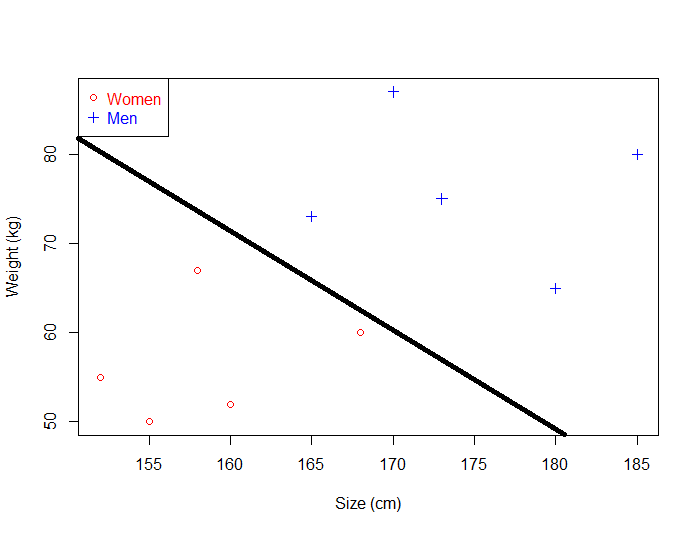
\includegraphics[width=0.9\textwidth]{svm.png}
	\caption{SVMs được dùng để phân lớp tập dữ liệu thành hai lớp phân biệt}
    \label{fig:svm}
\end{figure}

\paragraph*{}
Một siêu phẳng là một hàm tương tự như phương trình đường thẳng $y = ax + b$. Trong không gian hai chiều (2D), siêu phẳng chính là đường thẳng. Trong thực tế, để học các bộ phân lớp tuyến tính trên dữ liệu phức tạp, SVM ánh xạ tập dữ liệu ban đầu vào không gian nhiều chiều hơn. Khi đã ánh xạ sang không gian nhiều chiều, SVM sẽ xem xét và chọn ra siêu phẳng phù hợp nhất để phân lớp tập dữ liệu đó. 

\begin{figure}[h!]
	\centering
	\captionsetup{width=0.8\textwidth}
	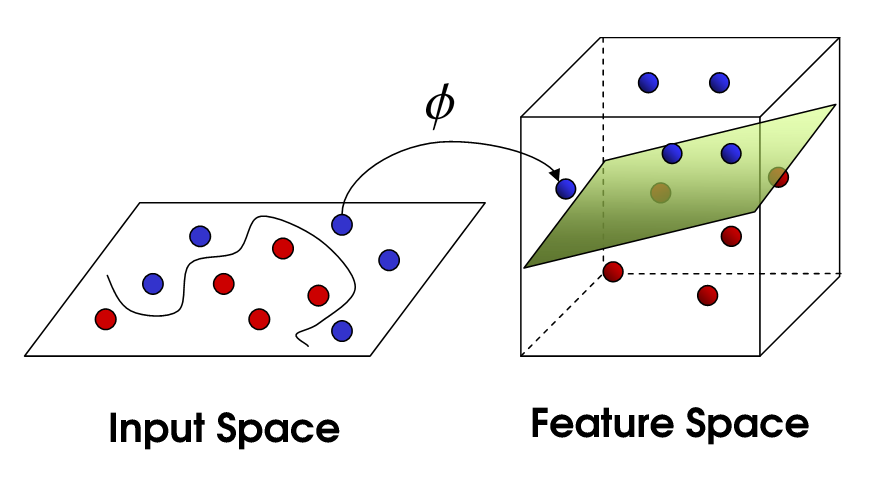
\includegraphics[width=0.9\textwidth]{svm_kernel.png}
	\caption{Dữ liệu được ánh xạ lên không gian cao hơn trước khi các bộ phân lớp được học}
    \label{fig:svm_kernel}
\end{figure}

\paragraph*{}
Hình \ref{fig:svm_kernel} là ví dụ cho phép ánh xạ này. Nếu chúng ta xem các chấm màu xanh và đỏ là những quả bong bóng, trong hình bên trái, các quả bóng này được đặt trên bàn, nếu chúng phân bố không quá đan xen vào nhau, ta có thể dùng một cây que dài để chia các quả bóng thành hai tập xanh và đỏ mà không động đến các quả bóng. Lúc này, khi đưa một quả bóng mới đặt lên mặt bàn, bằng cách xác định nó nằm bên phía nào của cây que, ta có thể dự đoán màu sắc của quả bóng đó. Các quả bóng tượng trưng cho các điểm dữ liệu, màu xanh và đỏ tượng trưng cho 2 lớp. Cái bàn tượng trưng cho một mặt phẳng. Cây que tượng trưng cho một siêu phẳng đơn giản đó là một đường thẳng. Tuy nhiên khi các quả bóng nằm đan xen nhau trên bàn (dữ liệu phức tạp hơn), lúc này không thể dùng cái que để phân tách chúng, để làm được điều này chúng ta cần hất các quả bóng bay lên (chính là phép ánh xạ), từ đó có thể sử dụng một tờ giấy để phân tách chúng (tờ giấy chính là siêu phẳng). Trên thực tế, SVMs thực hiện ánh xạ bằng việc sử dụng các kernel thích hợp. Việc lựa chọn kernel với các tham số thích hợp sẽ giúp SVM học được các bộ phân lớp tốt hơn trên những tập dữ liệu khác nhau

\subsection*{Margin}
Margin là một thuật ngữ quan trọng trong SVM chỉ khoảng cách giữa siêu phẳng đến 2 điểm dữ liệu gần nhất tương ứng với các phân lớp (\ref{fig:svm_margin}). Để có được bộ phân lớp tốt nhất, SVM cố gắng maximize margin này, từ đó thu được một siêu phẳng tạo khoảng cách xa nhất với hai lớp, nhờ vậy có thể giảm thiểu việc phân lớp sai (misclassification) đối với điểm dữ liệu mới đưa vào.

\begin{figure}[h!]
	\centering
	\captionsetup{width=0.8\textwidth}
	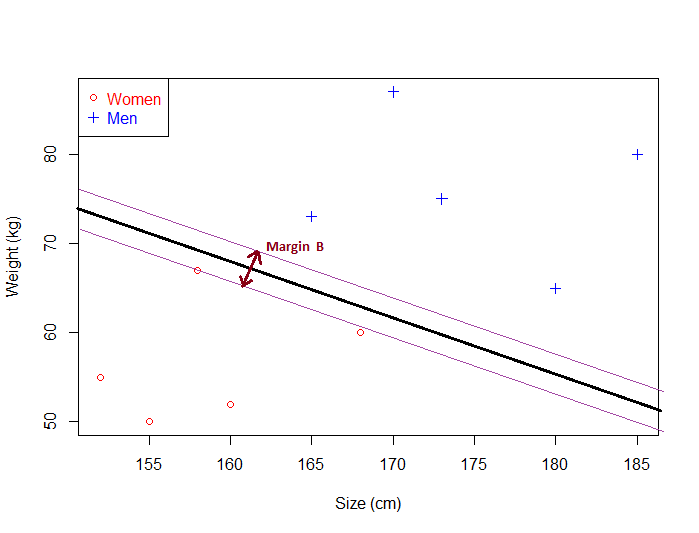
\includegraphics[width=0.7\textwidth]{svm_margin.png}
	\caption{Margin được maximize để giảm thiểu phân lớp sai cho dữ liệu mới}
    \label{fig:svm_margin}
\end{figure}

\paragraph*{}
Trong luận văn này, nhóm sử dụng SVM để huấn luyến các bộ phân lớp dựa trên các đặc trưng rút trích từ ảnh để phân lớp các loại vật liệu.

\section{Neural Network}

Neural Network là một loại hệ thống máy tính đặc biệt \cite{sampson1987parallel}, được lấy cảm hứng từ cấu trúc não của con người. Một tế bào trong não người được gọi là nơron có hai thành phần chính: Axons và Dendrites. Những tế bào thần kinh này hoạt động bằng cách xử lý các tín hiệu điện. Dựa trên tín hiệu nhận được thông qua Dendrites, Axons thực hiện mã hóa thần kinh (Neural coding) \cite{thorpe1990spike}, sau đó được phân phối tín hiệu này qua các Neurons và có thể được coi là đầu ra của hệ thần kinh. Axon của một Neuron được kết nối với Dendrites của Neurons khác, cứ như vậy các Neurons liên kết với nhau và hình thành Neurons Network trong não người (Hình \ref{fig:neuron}).

\begin{figure}[h!]
	\centering
	\captionsetup{width=0.7\textwidth}
	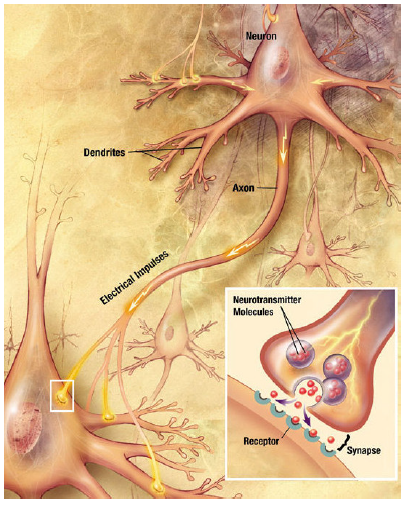
\includegraphics[width=0.5\textwidth]{neurons_network.PNG}
	\caption{Tín hiệu được truyền từ Axons của một neuron đến Dendrites của neuron tiếp theo}
    \label{fig:neuron}
\end{figure}

Với các tiến bộ trong khoa học máy tính, hiện nay chúng ta đã có thể phát triển hệ thống mạng hoạt dựa trên cách lan truyền tín hiệu của các nerouns trong hệ thần kinh. Thành phân cơ bản của hệ thống này là các nút (node) tương tác với nhau thông qua các trọng số và hàm lan truyền. Các node tương tự như các nerouns trong não. Một mạng neroun là sự kết hợp của nhiều layer của các node. Các layers được chia thành input layer, output layer và intermediate layer (còn được gọi là hidden layer). Đầu ra của mỗi node được tính toán thông qua hàm kích hoạt (activation function). Mỗi node gắn với mỗi giá trị trọng số (weight) và độ lệch (basis) riêng, hai giá trị. Trong nhiều trường hợp, mạng neroun là một hệ thống thích ứng (adaptive system) tự thay đổi cấu trúc của mình (các trọng số) dựa trên các thông tin bên ngoài hay bên trong đi qua mạng trong quá trình học.

\begin{figure}[h!]
	\centering
	\captionsetup{width=0.7\textwidth}
	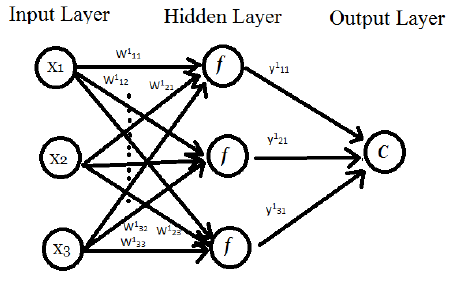
\includegraphics[width=0.5\textwidth]{single_layer_network.PNG}
	\caption{Cấu trúc của một Feedforward Perceptron Neural Network đơn giản.}
    \label{fig:simple_network}
\end{figure}

Hình \ref{fig:simple_network} là cấu trúc của một mạng neural đơn giản. Thuật ngữ "Feedforward" được dùng để chỉ cách dữ liệu đi qua mạng, trong trường hợp này dữ liệu chỉ đi qua mạng một chiều. Layer đầu tiên lấy các thông tin từ đầu vào, được gọi là input layer. Khi các giá trị đầu vào được truyền qua input layer, mỗi node sẽ tính toán giá trị output thông qua weights và biases, sau đó truyền output này tới hidden layer. Tại đây, các nodes dùng activation function để tính toán đầu ra rồi tiếp tục truyền tới layer cuối. Layer này được gọi là output layer, tính toán tất cả các "score" từ giá trị lan truyền từ layer trước. Với bài toán phân lớp, kết quả cuối cùng chính là lớp với giá trị "score" cao nhất sau khi qua output layer.

Giá trị đầu ra của mỗi node trong mạng được tính toán theo phương trình \ref{eq:simple_network}. Trong đó, $y_{j}$ là giá trị đầu ra của node thứ j của layer hiện tại, n là số lượng node của layer trước truyền thông tin vào node hiện tại, $f$ là hàm kích hoạt của node, $w_{mn}$ là trọng số được truyền từ node thứ m của layer trước đến node thứ n của layer hiện tại, $b_j$ là bias của node hiện tại (đang cần tính đầu ra)

\begin{eqnarray}
\label{eq:simple_network}
\hspace{1cm} y_{j} = f(\sum_{i=1}^{n} {w_{ij}x_i} + b_j)
\end{eqnarray}

Node đầu ra C sẽ nhận giá trị của các $y_j$ sau đó chọn lớp có score lớn nhất là output cuối cùng. Phương trình \ref{eq:y1}, \ref{eq:y2} và \ref{eq:y3} là cách tính giá trị đầu ra của từng node trong hidden layer
\begin{eqnarray}
\label{eq:y1}
\hspace{1cm} y_{1} = f(w_{11}x_1 + w_{21}x_2 + w_{31}x_3  + b_1)\\
\label{eq:y2}
\hspace{1cm} y_{2} = f(w_{12}x_1 + w_{22}x_2 + w_{32}x_3  + b_2)\\
\label{eq:y3}
\hspace{1cm} y_{3} = f(w_{13}x_1 + w_{23}x_2 + w_{33}x_3  + b_3)
\end{eqnarray}

Một hệ thống mạng neural với khả năng học tập hạn chế đã được phát triển trong công trình của Lugar và Stubble \cite{luger2005artificial} và được gọi là Perceptron. Mỗi node sẽ có đầu ra là 0 hoặc 1 được tính toán dựa trên một giá trị ngưỡng đặc biệt. Mạng neural này sẽ được học trên một tập dữ liệu huấn luyện. Mỗi mẫu trong tập huấn luyện gốm các giá trị đầu vào và giá trị đầu ra mong muốn tương ứng với nó. Các giá trị đầu vào được truyền vào input layer, đi qua mạng neural và cho một giá trị đầu ra (ở đây là 0 hoặc 1). Nếu giá trị đầu ra của mạng không giống với giá trị đầu ra mong muốn ban đầu thì giá trị các weights và thresholds sẽ được điều chỉnh để có kết quả tốt hơn. Hình \ref{fig:change_weights} là một cách thay đổi weights và thresholds để có kết quả tốt hơn.

\begin{figure}[h!]
	\centering
	\captionsetup{width=0.7\textwidth}
	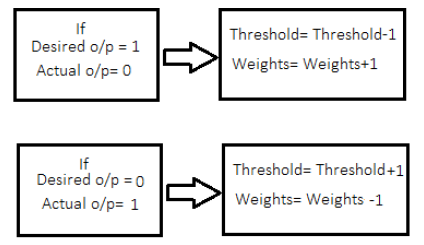
\includegraphics[width=0.5\textwidth]{change_weights.PNG}
	\caption{Một trong những cách đơn giản thay đổi weights và thresholds của một node để có kết quả tốt hơn}
    \label{fig:change_weights}
\end{figure}

Perceptron sau đó được phát triển thành mạng với nhiều hidden layer (multilayer). Cấu trúc này được học dựa trên thuật toán lan truyền ngược (backpropagation) \cite{sampson1987parallel}. Thuật toán này tuân theo quy tắc delta [\ref{widrow1960adaptive} để tính toán độ lỗi tại nút đầu ra. Độ lỗi của nút cuối cùng trong mạng (output node) được lan truyền ngược qua mạng sau mỗi lần huấn luyện, giá trị các weights sẽ 	được cập nhật dựa trên hàm lỗi. Cách học này còn được gọi là gradient descent. 
Giá trị đầu ra của một node phụ thuộc vào hàm kích hoạt và trong mạng lan truyền ngược là một hàm sigmoid (Phương trình \ref{sigmoid_function}) với $f_{j} = \sum_{i=1}^{n} {w_{ij}x_i}$

\begin{eqnarray}
	\label{eq:sigmoid_function}
	\hspace{1cm} \sigma(f_x) = \frac{1}{1 + e^{-f_x}}
\end{eqnarray}

Hàm sigmoid áp dụng cho tất cả các node trừ các input node và giá trị đầu ra được giới hạn trong khoảng [0,1].

\section{Convolutional Neural Networks (CNNs)}
Convolutional Neural Networks (CNNs) là một loại Neural Network đặc biệt. Nguyên tắt hoạt động của CNNs tương tự như một Neural Network bình thường: lấy input tại input layer, truyền giá trị này qua các hidden layer, dùng activation function tính toán giá trị đầu ra tại mỗi node. Score tại các node ở layer cuối (output layer) được lan truyền ngược và các trọng số của mạng được cập nhật sau mỗi lần huấn luyện. Trong thực tế, CNNs khó huấn luyến hơn các Neural Network bình thường do sự phức tạp của nó.Nhưng điều gì khiến CNNs đặc biệt hiệu quả trong các vấn đề của Thị Giác Máy Tính? Hãy cùng tìm hiểu bên dưới.

Các Neural Network bình thường không thích ứng tốt với các ảnh đầu vào khác nhau. Với ảnh đầu vào 32x32 RGB, input layer sẽ có $32*32*3 = 3072$ weights. Nhưng trên thực tế, kích thước của ảnh đầu vào lớn hơn nhiều, cho một ảnh với kích thước 600x300 RGB, sẽ có tới $600*300*3 = 540000$ weights chỉ tính input layer - một con số không hề nhỏ! Để khắc phục điều này nhận cả bức ảnh làm đầu vào. Năm 2012, CNNs bắt đầu nhận được sự chú ý của nhiều nhà nghiên cứu trong lĩnh vực phân lớp ảnh khi Alex Krizhevsky thắng giải trong cuộc thi của Imagenet bằng việc thiết kế một mạng CNN và giảm độ lỗi trong việc phân lớp đối tượng từ 26.2\% xuống còn 15.3\% \cite{krizhevsky2012imagenet}. CNN tận dụng lợi thế của bất kỳ cấu trúc đầu vào nào thể hiện mối tương quan không gian (chẳng hạn như hình ảnh) và sắp xếp các neural theo không gian này. Sự sắp xếp này cho phép thông tin đi qua mạng hiệu quả và giảm đáng kể số lượng tham số của mạng. Cấu trúc của một mạng CNN gồm nhiều phần khác nhau: Convolutional Layer, Pooling Layer, Rectied Linear Unit hoặc ReLU Layer và Fully Connected Layer. Một trong những kiến trúc CNN cơ bản (LeNet-5) \cite{lecun1998gradient} dùng cho nhận diện chữ viết được thể hiện trong hình \ref{fig:lenet_5}

\begin{figure}[h!]
	\centering
	\captionsetup{width=0.7\textwidth}
	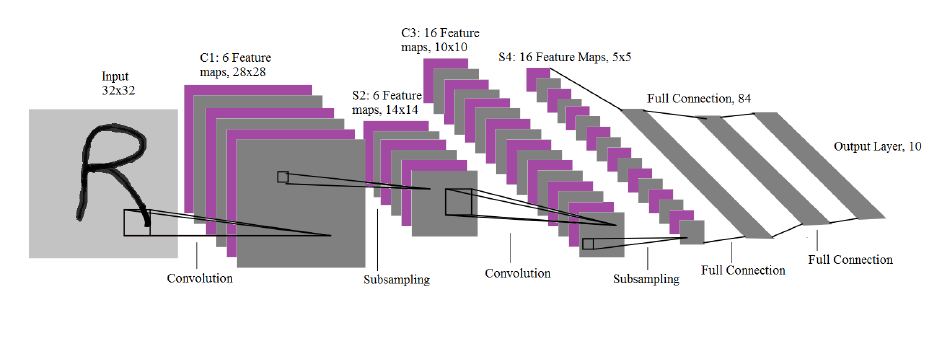
\includegraphics[width=1.0\textwidth]{lenet_5.PNG}
	\caption{Cấu trúc mạng LeNet-5, một mạng CNN dùng cho nhận diện chữ viết}
    \label{fig:lenet_5}
\end{figure}

\subsection*{Convolutional layer}
Convolutional layer là thành phần chính thực hiện hầu hết các tính toán trong một mạng CNN, Mỗi convolutional layer chứa một tập các filters (hay kernels) với kích thước ứng với các weights và biases. Trong quá trình lan truyền của một mạng CNN, mỗi kernel trượt qua tất cả các vùng của ảnh đầu vào và thực hiện phép toán dot product trên mỗi vùng đó. Mỗi kernel rút trích các đặc trưng khác nhau từ ảnh. Các phép toán này làm giảm dần số chiều (kích thước) của đầu vào nhưng cũng làm tăng độ sâu của mạng.

Ba tham số quyết định đầu ra của một convolutional layer bao gồm: depth, stride và zero-padding. \textbf{Depth} thay đổi đầu ra của convolutional layer dựa vào số lượng kernel của layer đó. Số lượng kernel càng lớn thì đầu ra của layer sẽ càng "sâu". \textbf{Stride} là tham số thể hiện bước nhảy của kernel khi trượt trên ảnh để thực hiện dot product. Nếu stride có giá trị là 1 thì kernel se trượt một pixel sau mỗi phép dot product. Bằng cách này, stride sẽ quyết định kích thước của đầu ra. \textbf{Zero-padding} cũng ảnh hưởng đến kích thước của đầu ra thông qua việc thêm 0 vào các cạnh của ảnh hay ma trận đầu vào. 

\begin{figure}[h!]
	\centering
	\captionsetup{width=0.7\textwidth}
	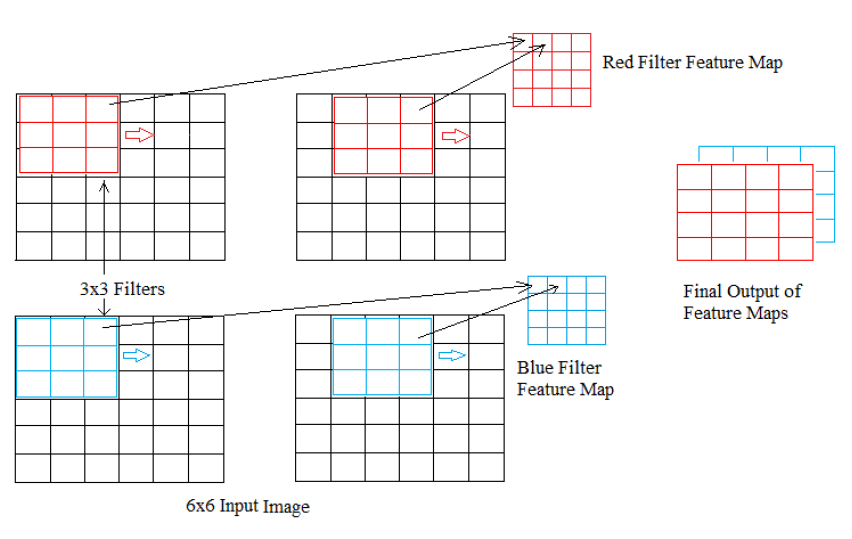
\includegraphics[width=1.0\textwidth]{filters.PNG}
	\caption{Hai filter 3x3 được dùng để tính toán hai 4x4 2D feature map từ một ma trận đầu vào 6x6}
    \label{fig:filters}
\end{figure}

Hình \ref{fig:filters} thể hiển quá trình tính toán của một convolutional layer sử dụng 2 filters 3x3 cho ma trận đầu vào 6x6 (không dùng zero-padding). Sau khi các phép toán dot product hoàn thành, kết quả đầu ra của layer này là hai 2D feature map 4x4 (hay có thể nói đầu ra có kích thước 4x4x2). Đây chính là ví dụ cho việc giảm kích thước đầu vào nhưng tăng chiều sâu của layer trong mạng CNN. Một cách tổng quát, với ma trận đầu vào kích thước NxN đi qua một convolutional layer với Y filters MxM (stride = 1 và không dùng zero-padding) thì đầu ra có kích thước (N - M + 1) X (N - M + 1) X Y

\subsection*{Pooling Layer}
Là một loại layer quan trọng khác trong CNN, pooling layer thường được dùng ở giữa hai convolutional layers. Pooling layer được dùng để giảm kích thước của ma trận đầu vào (vì vấy nó còn có tên khác là downsampling layer). Kiểu pooling layer phổ biến nhất là max pooling layer, thường sử dụng với filter có kích thước 2x2 và stride = 2 pixels. Hình \ref{fig:max_pooling} cho thấy tác dụng của layer này, giảm kích thước ma trân đầu vào từ 4x4 xuống còn 2x2.

\begin{figure}[h!]
	\centering
	\captionsetup{width=0.7\textwidth}
	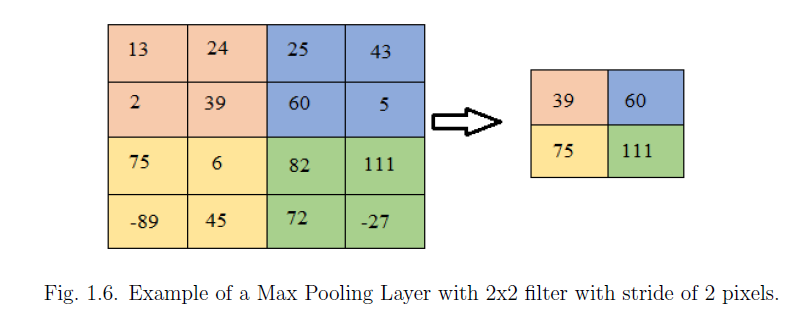
\includegraphics[width=1.0\textwidth]{max_pooling.PNG}
	\caption{Một max pooling layer với filter 2x2 và stride = 2 pixels}
    \label{fig:max_pooling}
\end{figure}

Những phương pháp gần đây thường không dùng pooling layer ở giữa hai convolutional layer. Thay vào đó, để đạt được tác dụng tương tự pooling layer (giảm kích thước), stride của convolutional layer thường được dùng với giá trị cao hơn \ref{springenberg2014striving}.

\subsection*{ReLU (Rectied Linear Unit) Layer}
Rectied Linear Unit hay ReLU layer thường được dùng sau convolutional layer và trước pooling layer. Thực nghiệm cho thấy layer này được dùng để tăng hiệu quả tính toán của mạng CNN [16].
ReLU layer không thay đổi kích thước của ma trận đầu vào. Trong ví dụ Hình \ref{fig:relu}, layer này sử dụng hàm $f(x) = max(0, x)$ để thay đổi tất cả các giá trị âm thành 0.

\begin{figure}[h!]
	\centering
	\captionsetup{width=0.7\textwidth}
	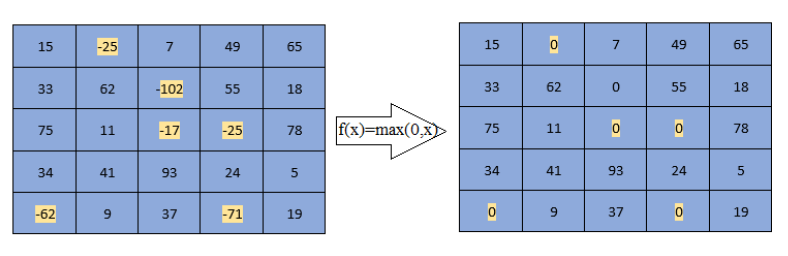
\includegraphics[width=1.0\textwidth]{relu.PNG}
	\caption{ReLU layer sử dụng hàm $f(x) = max(0, x)$ để thay đổi tất cả các giá trị âm thành 0}
    \label{fig:relu}
\end{figure}

\subsection*{Fully Connected Layer}
Fully connected layer được dùng như layer cuối cùng của một mạng CNN (output layer). Tại đây, mỗi node trong layer trước liên kết với tất cả các node của layer tiếp theo, Layer này được dùng để chuyển đổi feature map từ layer trước thành classification score.

\section{Transfer Learning}
Với bài toán phân lớp ảnh, để đạt kết quả tốt đòi hỏi một cấu trúc mạng thích hợp, điều này phụ thuộc nhiều vào tập dữ liệu huấn luyện. Trong thực tế, dữ liệu huấn luyện rất lớn và đa dạng. Một cấu trúc mạng tốt có thể học được khối lượng dữ liệu lớn thường rất phức tạp và đòi hỏi khá nhiều về phần cứng để thực hiện huấn luyện. Alexnet \cite{krizhevsky2012imagenet} sử dụng hơn 1.2 triệu ảnh thuộc 1000 lớp khác nhau để huấn luyện trên hai GTX 580 3GB GPUs trong gần một tuần.

Với các bài toán trên tập dữ liệu khác, kỹ thuật transfer learning được dùng để sử dụng lại các mạng phức tạp đã được huấn luyện sẵn này, và chỉ huấn luyện lại một phần nhỏ để thích hợp với bài toán mới. Cách tiếp cân này đã được được rất nhiều kết quả tốt trong nhiều bài toán phân lớp trên những tập dữ liệu khác nhau.

Một cách đơn giản nhưng hiểu quả để áp dụng kỹ thuật này là sử dụng lại toàn bộ một mạng CNN được train trên tập dữ liệu lớn, thay layer cuối cùng bằng một Softmax Regression nhưng với số lượng units bằng với số lượng class ở bộ cơ sở dữ liệu mới và chỉ huấn luyện lại tham số cho layer này để giảm thiểu chi phí tính toán và thời gian

Ngoài ra, chúng ta cũng có thể sử dụng feature map ở những layer gần cuối (fully connected layers) rút ra từ các mạng được huấn luyện sẵn như một feature (deep feature) và sử dụng các thuật toán máy học như SVMs (Support Vector Machines) để huấn luyện các bộ phân lớp cho bài toán mới.